
\thispagestyle{empty}
\vspace*{0.30\textheight}
\begin{quote}\kaishu
  我可以借一颗待开的坚果的……意象，来说明这种……做法。我起初想到的比喻是：
  把坚果浸到某种软化的液体里——为什么不干脆就用清水呢？不时搓一搓，好让
  液体渗得更透，其余便交给时间。几个星期、几个月过去，壳渐渐变软——时机
  成熟的那一刻，手掌一按便足矣，壳会像熟透的牛油果那样应声裂开！……

  几个星期前浮现在我眼前的意象又自不同。那件有待认识的未知之物，在我看来
  像是一片土地，或某种致密的泥灰岩，抗拒着被穿透。……大海悄然无声地向前
  推进，似乎什么都没有发生，什么都没有动，水离得那么远，几乎听不见。……
  然而它终究将那倔强的实体拥入怀中。
\end{quote}
\vspace{1em}
\begin{flushright}\kaishu\small
  ——A.~\trGrothendieck，[Gr5, pp.~552--3]；英译 C.~\trMcLarty，[Mc, p.~1]\footnote{译注：本书书名「上涨的海」即典出于此。}
\end{flushright}
\vspace{2em}
\clearpage

\chapter*{前言}
\addcontentsline{toc}{chapter}{前言}
\markboth{前言}{}%
\setcounter{chapter}{0}

本书旨在给出\trAlgebraicGeometry{}的一个严肃且相当完整的引论，而它不只是写给本领域的（未来）专家的。全书的讲法服务于一组明确而有限的目标（见 \S0.4），因而不可避免地采取关于这门学科的某一特定视角。

大卫·\trMumford{}写下如下这段话，已是几十年前的事了：代数几何“似乎背上了玄奥、排外、极度抽象的名声，其信徒暗中密谋接管数学的其余全部领域！就最后这一点而言，他们没有说错”（[Mu4, preface] 与 [Mu7, p.~227]）。如今这场革命已然全面成真，并从根本上改变了我们对纯粹数学诸多领域的思考方式。数量惊人的著名进展，都以这样或那样的方式，依赖于亚历山大·\trGrothendieck{}、让-皮埃尔·\trSerre{}等人率先阐明的洞见与思想。

出于种种原因，\trAlgebraicGeometry{}落下了「难以企及」的名声。这门学科的力量来自颇为抽象的重型机械，而其对象与方法的直观本性，却容易因此被遮蔽。邻近领域的许多人，对这门学科的基本思想只有一个模糊的印象。\trAlgebraicGeometry{}本身也已裂解为诸多分支；即便身在代数几何之内，新的研究者对远离自身方向的子领域中的基本思想，往往也一无所知。

但还有一种更乐观的看法。\trAlgebraicGeometry{}赖以贯通数学多个部分的思想是基础的，动机也是充分的。邻近领域的许多人会发现：对这门学科的基础发展出一套能上手运用的知识是有益的，而且不应止于皮毛。在代数几何内部，存在一部「\trCanon{}」（canon）——至少对从这个特定方向接近这门学科的人而言如此——领域中的每个人都能够、也应当熟悉它。\trSchemeTheory{}的毛糙棱角，在过去的半个世纪里已经打磨光滑；尽管如此，按这门学科自身的门道去理解它，仍是无可回避的功课。

\noindent\textbf{0.0.1. 练习的重要性。}\quad 本书的练习非常多。我的经验是：若没有几个可供自己反复思索的问题，思想便无法在心里扎根。有些练习是平凡的——某些专家对此颇为反感，我却觉得这正是可取之处。极少数必要的练习可能相当难，但读者理应已被授予应对它们的背景知识——把难题放进练习，并不只是把硬核材料从正文里推出去的借口。练习穿插于讲述之中，而不是堆在各节末尾。绝大多数练习都经过了课堂上的反复检验。

这里采取的立场，是我与\trKedlaya、\trPoonen{}在 [KPV] 中一同探索过的：那本书表面上谈的是问题，骨子里却是一份关于「应当如何学习、思考与做数学」的申论。多数人靠动手来学，而不只是被动地读。挑选得当的问题，可以是引导学习者走向觉悟的最好方式。

\noindent\textbf{0.0.2. 编号结构。}\quad 你很快会注意到，所有条目都按 x.y.z 编号：x 是章号，y 是节号，z 是一个数字——唯独练习用字母标示（并且穿插于全书正文之中，而不是放在各节末尾）。单个段落也常常带有编号，以便引用，或标示一个新话题。定义以粗体排印，有时是顺带给出的。

\section{致读者}

本书旨在汇集一群人的共同智慧，而这智慧必然是经由一个不完美的滤器蒸馏而来。关于你可能如何使用本书，我想说几句话——不过这些建议是否值得听从，我自己也不清楚。

在讨论细节之前，我想先把一句话说在开头：现代代数几何这台美妙的机器，本是为了理解关于几何（取其广义）的那些基本而朴素的问题而被创造出来的。本书的目的，就是让你在这些强有力的思想上打下扎实的根基。不要被「食莲人」%
\footnote{译注：lotus-eaters，典出《奥德赛》；吃了忘忧莲的人乐不思蜀，忘却归途。}
诱入对无所依凭的抽象的迷恋；在学习这些已被证明对研究基本问题极为有效的形式结构时，请牢牢抓住你的几何动机。接触一个新思想时，永远要问：我为什么要关心它？不要指望立刻得到答案，但要坚持最终得到答案。至少要试着把每一个新抽象，应用到某个你能透彻理解的具体例子上。看看你能否画一张粗糙的图，捕捉住该思想的本质。（书中大多数插图，是我特意请一位手脚不协调、一脸茫然的三岁小孩画的，以表明哪怕是潦草的速写，也能启发人、澄清事理。）

人们常以为代数几何难懂，是因为它由大而复杂的机械部件构成。事实恰恰相反；换个比喻说，代数几何并不窄而深，而是浅却极广。它由大量非常小的部件搭建而成，正合\trGrothendieck{}对数学的构想。要把这个有机整体——连同其纷乱的相互勾连——整个装进脑子，是一项挑战。

一个合理的起点，是「\trAffine\trComplex\trVariety{}」（affine complex variety）的观念：由若干多项式方程从 $\mathbb{C}^n$ 中切出的子集。你的几何直觉立刻就能派上用场——关于\trDimension、\trSmoothness，或诸如 $\mathbb{R}$、$\mathbb{Q}$ 这类子域上的解，你也许已有一肚子想法或疑问。更有智慧的人会建议：先花些时间把复簇理解得足够细致，再去学概形。我却要反过来鼓动你：立刻去学概形，把\trAffine\trComplex\trVariety{}当作中心的（但非唯一的）例子来学习。这并不理想，却能节省时间，而且出人意料地行得通。另一条路是先在别处学习簇，日后再回到本书。

概形的直观，可以建立在仿射复簇的直观之上。\trKnutson{}与\trTao{}指出，这一步同时包含三个不同方向的推广，可视为数学中三个宏大的主题：(i)~我们允许函数环中有\trNilpotent{}元，这基本上是\trAnalysis{}（考察方程的近似解而非精确解）；(ii)~我们把这些\trAffine\trScheme{}粘合起来，这正是\trDifferentialGeometry{}中的做法（考察\trManifold{}而非\trCoordinatePatch{}）；(iii)~我们不再于 $\mathbb{C}$（或其他\trAlgClosedField{}）上工作，而是在更一般的、不是代数闭域甚至根本不是域的环上工作，这基本上是\trNumberTheory{}（在数域、整数环等之上求解方程）。

由于我们的目标是全面，是要把一门初等课程之后你应当知道的一切都讲明白，到达有趣的示范性应用必然要花更长时间。你也许会误以为：要抵达这些应用，非得下这么大的苦功不可——并非如此！你应当有意识地留心那些你从前就会在意的例子。这需要一些时间与耐心。

在学习代数几何的过程中，你应当留意那些关键的垫脚石。当然，越往前走，步子就越大。

\noindent\textbf{第 1 章。}\quad 范畴论只是语言，但它是内嵌了逻辑的语言。一旦意识到范畴论的使命是把你已经知道的东西形式化、抽象化，它就会容易得多。开头这章范畴论，是要训练你把思路理干净。举例来说，当有人把某个东西命名为「\trCokernel{}」或「\trProduct{}」时，你应当想知道它凭什么配得上这个名字，以及这个名字本应意味着什么。这种思考方式在观念上的优势，会随时间推移逐渐显现。\trYonedaLemma{}——以及更一般的「通过映到对象的态射来理解对象」的思想——将扮演重要角色。

\noindent\textbf{第 2 章。}\quad \trSheaf{}的理论再次把某件你早已充分理解的东西抽象化（见 \S2.1 的引例）；困难之处在于理解如何最好地打包与运用一个层的信息（\trStalk、\trSheafification、\trBase{}上的层，等等）。

第 1、2 章是一场冒险的赌局，它们试图维持一种微妙的平衡。讲解代数几何的书，常常把这类背景丢给读者自行补足，让读者去查他们根本不会去查的其他文献，或者把它塞进一份电报体附录。本书反其道而行之：凡必要者都试图讲清，但也仅以必要为限；并且力求传达你应当如何思考（以及运用）这些基本思想，以及它们为什么比你担心的更有根基。

\noindent\textbf{第 3--5 章。}\quad 备好这份背景之后，你就能清清爽爽地思考几何各领域所研究的形形色色的「空间」——包括实\trManifold、\trTopologicalSpace{}与复流形——它们都是局部具有某种特定形态的\trRingedSpace{}（ringed space）。\trScheme{}不过是又一种「几何空间」；于是我们便可以把大量来自「经典几何」的直观搬进这个新舞台。（这也为你日后思考代数几何中其他类型的几何空间做好了铺垫，例如\trComplexAnalyticSpace、\trAlgebraicSpace、\trOrbifold、\trStack、\trRigidAnalyticSpace{}与\trFormalScheme。）概形与你的几何直觉相悖之处，是可以内化的，你的直觉也可以扩展到把它们容纳进来。你会意识到自己想要的性质有许多，还有一些性质日后会被证明是重要的。它们都配拥有名字。请不慌不忙地与它们一一熟络起来。

\noindent\textbf{第 7--11 章。}\quad 以范畴的方式思考，会引你去追问概形（以及几何中的其他空间）的\trMorphism。\trGrothendieck{}的一条根本教诲是：态射才是核心。重要的几何性质，归根结底应当理解为态射的性质。有许多带专名的态射类；对每一类，你都应当想清楚它凭什么配上这个名字。

\noindent\textbf{第 12--13 章。}\quad 到那时，你将处于一个有利的位置，去思考概形的基本几何性质：\trDimension{}与\trSmoothness。这些观念竟如此微妙，你也许会吃惊；但请记住，在数学的任何地方它们都是微妙的。

\noindent\textbf{第 14--22 章。}\quad \trVectorBundle{}是几何中无处不在的工具，代数几何也不例外。它们把我们引向更一般的\trQCSheaf，正如环上的自由模把我们引向更一般的\trModule。接下来我们研究它们的性质，包括\trCohomology。第 19 章把这些思想应用于曲线的研究，或许能让你看清它们究竟多么有用。

\noindent\textbf{第 23--29 章。}\quad 手握这些，你就可以去学习本学科广泛使用的更高级的工具了。书中给出大量「你能做什么」的例子；光滑三次曲面上的 27 条直线这一经典故事（第 27 章），正是看众多思想汇聚一堂的好机会。

各章之间粗略的逻辑依赖如图~0.1 所示。（当心：这张图只能姑妄听之。例如，你应当避免在后文各章大量使用第 19 章的曲线理论；但它是例子的重要来源，也是巩固理解的好办法。）

\begin{figure}[htbp]
  \centering
  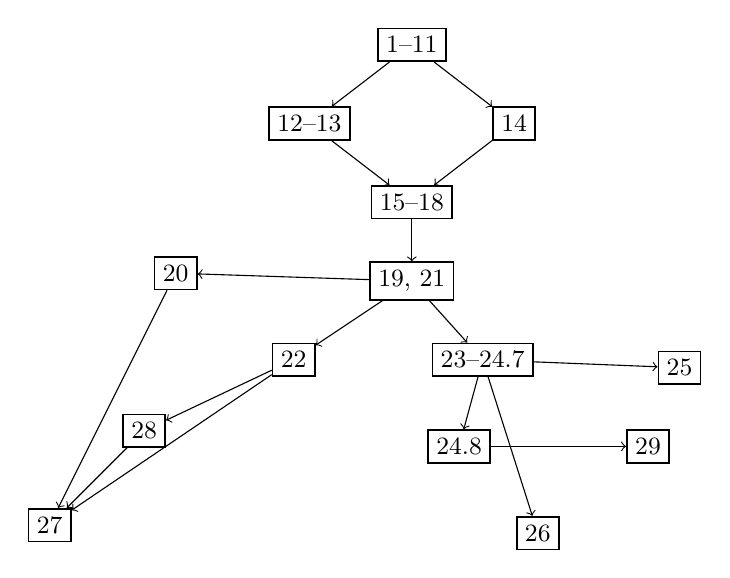
\begin{tikzpicture}[vbox/.style={draw,semithick,inner sep=3pt,font=\small}]
    \node[vbox] (a) at ( 0.0, 0.0) {1--11};
    \node[vbox] (b) at (-1.3,-1.0) {12--13};
    \node[vbox] (c) at ( 1.3,-1.0) {14};
    \node[vbox] (d) at ( 0.0,-2.0) {15--18};
    \node[vbox] (e) at (-3.0,-2.9) {20};
    \node[vbox] (f) at ( 0.0,-3.0) {19,~21};
    \node[vbox] (g) at (-1.5,-4.0) {22};
    \node[vbox] (h) at ( 0.9,-4.0) {23--24.7};
    \node[vbox] (i) at ( 3.4,-4.1) {25};
    \node[vbox] (j) at (-3.4,-4.9) {28};
    \node[vbox] (k) at ( 0.6,-5.1) {24.8};
    \node[vbox] (l) at ( 3.0,-5.1) {29};
    \node[vbox] (m) at (-4.6,-6.1) {27};
    \node[vbox] (n) at ( 1.6,-6.2) {26};
    \draw[->] (a)--(b); \draw[->] (a)--(c);
    \draw[->] (b)--(d); \draw[->] (c)--(d);
    \draw[->] (d)--(f);
    \draw[->] (f)--(e); \draw[->] (f)--(g); \draw[->] (f)--(h);
    \draw[->] (h)--(i);
    \draw[->] (g)--(j);
    \draw[->] (h)--(k);
    \draw[->] (k)--(l);
    \draw[->] (e)--(m); \draw[->] (g)--(m); \draw[->] (j)--(m);
    \draw[->] (h)--(n);
  \end{tikzpicture}
  \caption{各章之间的重要逻辑依赖（更确切地说：一张有向图，指出哪一章应当先于哪一章阅读）。}\footnote{依原书手绘图重绘，个别箭头或有出入。}
\end{figure}

总的说来，我偏好尽可能少的假设。对证明并非必需的假设，无异于转移视线的红鲱鱼。但若一个合理的假设能让证明更干净、更令人难忘，我也乐于把它写进去。

特别地，\trNoetherian{}假设在必要时很顺手，此外则有误导之嫌。即便是一心只想着诺特的读者（即正常人），在正确的假设下也会有收获——它们会把「事情为什么成立」讲得更清楚。

我常常陈述仅对\trVariety{}成立的特别结果，尤其当这一情形有独到的、值得掌握的技巧时。但令人意外的是，把论域限制在\trAlgClosedField{}上其实很少有用。几何学家不必惧怕算术例子或代数例子；代数几何的一个核心洞见正是：同一套形式体系原封不动地适用。

病态的例子值得认识。山区公路两旁立着为坏天气准备的高杆：冬日里你看不清路面，高杆便是警示——越过这条线，你就没命了！病态与（反）例子服务于类似的目的。当你面对一个拿不准真伪的新命题、定理或猜想时，它们也是现成的试金石（例如见 \S4.1.8）。

攻读一本代数几何的书时，手边备着另外几本代数几何书格外有用：可以看看不同的进路，在遇到困难时也有别的去处。本书可以作为一本不错的辅读书。若它就是你的主教材，那么还有两本在我看来哲学相近的优秀著作：[Liu] 与 [GW]。\trDeJong{}的百科全书式在线参考 [Stacks] 则是无出其右的。此外还有许多出色的材料，也许每一种进路都对应一本；你应当四处翻翻，找到与你投缘的那一本。

若你想找的是这门学科一部正确或完整的历史，那你来错了地方。本书无意成为文献的完备指南；由于我自己的无知与懒惰，许多重要的文献来源被忽略或遗漏了。

最后，若你试图不做过相当数量的练习（见 \S0.0.1）就读完本书，我会亲自登门，用 [Gr-EGA] 把你揍到求饶为止。只对「什么是真的」有个模糊印象是不够的，你得能真刀真枪地把手弄脏。借用\trKisin{}的话：“手挥得再花哨也没用，你还是飞不起来。”注：书末的提示也许帮得上忙，但有时未必。

\section{致行家}

若你把本书用作课程教材，自然应当按照你自己的视角与兴趣来取舍。特别地，你应当想好一个希望在课程结尾抵达的应用或定理（它很可能不在本书之中），然后朝它进发。你不必强求冲刺到全书终点；我反倒建议多花些时间，在最合适于你的学生的地方收束。（图~0.1 标出了各章之间大尺度的依赖关系，或许能帮你规划课程。）据我的经验，曲线论（第 19 章）与三次曲面上的 27 条直线（第 27 章）作为冬、春学季末尾的目标，效果一向很好；即便所需的某些背景没有来得及讲、学生只能把它当作某种黑箱，也依然如此。第一个学季的目标，是为多种几何与几何空间（不只是代数几何，还有流形、\trComplexGeometry、一些\trDifferentialGeometry{}等等）建立一套共同语言——某种「几何空间」的原型形态。

忠实于 \S0.4 的目标，需要进行一场残酷的取舍；我做了不少你或许想推翻的决定。下面简述其中一些可能有争议的选择。

在「如何讲述」上的取舍，是为学习者着想而做的。若有两个进路，一个从高观点看「正确」，另一个从朴素的立场看直接而自然，我选后者。

另一方面，\trVarietyTheory{}（比如在\trAlgClosedField{}上的）没有先行单独讲述。这个决定曾让我几欲落泪，但最终我确信：只要把握正确的精神，它是行得通的。

我没有把课程的第一部分花在簇上，而是把时间用在别处。一种诱人的想法是：学生要么早已对范畴论与层论驾轻就熟，要么会在课余自行把这些思想捡起来。但愿我生活在那个世界里。我劝你不要在这些基础问题上偷工减料。我的体会是：尽管头几讲在我自己看来慢得令人痛苦，但对不少学生却是启示性的；经验较多者也不觉得无聊，并未浪费时间。当我能够指望他们思路干净、并在实践中运用这些工具时，这份投资得到了成倍的回报。何况，就算他们离开课程时除了一手操作这些思想的经验之外一无所获，世界也因之更好了一点。

大体上，我们把结果陈述到证明所能支撑的最大一般性；但若更强结果的一般性根本不会被用到，我们不会为此付出艰难得多的证明。少数几处，我们下了更大的力气去证明某个更一般的结果，许多读者未必领情。例如，我们证明了若干定理对\trProper\trMorphism{}（而不只是\trProjective\trMorphism）成立。但在这类场合，我们邀请乃至鼓励读者，无视为更大一般性所付出的那些微妙代价。

我认为，\trLineBundle{}（以及到\trProjectiveSpace{}的映射）比\trDivisor{}更为根本。一般的\trCartierDivisor{}不会被严肃讨论（\S15.6.4），尽管\trEffectiveDivisor{}扮演着关键角色。

\trCohomology{}先用\trCech{}的办法来做（正如\trSerre{}当年所做），\trDerivedFunctor{}上同调只在后来才引入。我十分清楚，\trGrothendieck{}认为\trCechCohomology{}与导出函子上同调的一致「应当被看作一个偶然现象」，并且「出于技术上的理由，重要的是不要采取这个[切赫]上同调定义」（[Gr3, p.~108]）。但我确信，对多数人而言，这是初次见识这种上同调的正确方式。（诚然，代数几何中的许多主题，用导出函子的语言理解起来最好。但那是自山巅俯瞰的风景，并不是探察森林的最好方式。要恰当地领会导出函子，你必须理解其背后的\trHomologicalAlgebra，而不能只把它当成黑箱。）

只在必要时（或确能省力的少数场合），我们才限制在\trNoetherian{}情形。这样，非诺特阵营的人会清楚看到自己须在何处当心，而诺特阵营的人也会明白非诺特的东西并非那么可怕。何况，即使你主要关心的是诺特概形，让「诺特」只在必要时出现在定理的假设里也有好处——这会帮你记住这条性质究竟在何时、以何种方式被用到。

在某些场合，诺特读者会比本来要多受一点罪。举一个「火上浇油」的例子：我们不用诺特假设，而是又早又勤地请出\trQuasiseparatedness。代价是，在一大堆已令人应接不暇的词语之外，还得再多记一个词。可一旦记住了，便不难想到：凡有人关心的概形，几乎都是拟分离的。况且，无论何时，只要“\trQuasicompact{}且\trQuasiSeparated”这组假设出现，读者立刻就能猜到证明的关键想法。再举一例：在诺特情形下，\trCoherentSheaf{}与\trFiniteType{}（拟凝聚）层并无二致，但出于同样的理由——把证明里真正用到的东西讲清楚——在定理与练习的陈述中仍值得把它们区分开来。

许多重要的专题没有讨论。\trValuativeCriteria{}未予证明（见 \S13.7），其陈述被降格放进一节选读内容。完全略去的主题有：分层拼装的论证艺术（d\'evissage）、\trFormalScheme，以及带支撑的\trCohomology。抱歉了！

\section{背景与约定}

\epigraph
  {“只当个代数学家，还是只当个几何学家？”这样的问法，就像在问：“你宁可聋，还是宁可瞎？”}
  {——M.~\trAtiyah，[At2, p.~659]}

如无明确声明，所有的\trRing{}都假定为\trCommutative{}环，且都含有\trUnit，记作 1。环的映射必须把 1 映到 1。我们不要求 $0\neq 1$；换言之，「\trZeroRing{}」（只有一个元素的环）也是环。（从任何环到零环都有环映射；零环只映射到它自身。零环是环范畴中的\trFinalObject。）「\trIntegralDomain{}」的定义包含 $1\neq 0$，因此零环不是整环。我们接受\trAxiomOfChoice，通常以\trZornsLemma{}的面目出现。特别地，环中的任何\trProperIdeal{}都包含在某个\trMaximalIdeal{}之中。（「$A$-模范畴有足够多\trInjective{}对象」的论证也用到选择公理；见练习~23.2.G。）

读者应熟悉\trCommutative{}环论的若干基础：特别是理想的概念（包括\trPrimeIdeal{}与\trMaximalIdeal）、各种类型的环（包括\trIntegralDomain、\trPID、\trUFD{}与\trLocalRing）、\trLocalization，以及\trModule。$A$-模的\trTensorProduct{}与\trExactSequence{}将是重要的。局部环（有唯一极大理想的环）将使用记号 $(\Lambda,\mathfrak{m})$ 或 $(\Lambda,\mathfrak{m},k)$——$\Lambda$ 是环，$\mathfrak{m}$ 是其极大理想，$k=\Lambda/\mathfrak{m}$ 是\trResidueField。我们会使用\trPID{} $\Lambda$ 上有限生成模的结构定理：任何这样的模都可写成主模 $\Lambda/(\alpha)$ 的\trDirectSum。域论的某些经验，也会不时派上用场。

\trManifold{}会作为例子不时登场，但它们多半只用于激发动机，因此我们通常不去指明究竟是哪一种：拓扑的（实流形）、\trDifferentiable{}的（$C^\infty$，即\trSmooth{}的）实流形、\trAnalytic{}的（实）流形，还是\trComplex{}的（\trHolomorphic{}）流形。尽管如此，这四种我们都会给出定义（定义~4.3.9）。

\noindent\textbf{0.3.1. 关于基础问题的警示。}\quad 我们不去操心那些微妙的基础问题（\trSetTheoretic{}问题、\trUniverse{}等）。的确，有些人应当在这些问题上小心翼翼。可你真的想那样过日子吗？（若你正是这类稀有之人，一个不错的起点是 [KS2, \S1.1]。）

\noindent\textbf{0.3.2. 更多的背景。}\quad 手边备几本其他学科的书，遇到具体事实时翻检一下，要好于提前通读。\trCommutative{}代数方面，[E] 正适合此用；流行的选择还有 [AtM] 与 [Mat2]。[Al] 采用的视角对代数几何很有用。\trHomologicalAlgebra{}方面，[Weib] 既详尽又好读。

来自数学其他部分（拓扑、几何、复\trAnalysis、\trNumberTheory{}……）的背景，当然有助于建立直观与根基。此前接触过一点拓扑，无疑是必不可少的。

\noindent\textbf{0.3.3. 非数学的约定。}\quad 「不重要」意指「对眼下的讲述不重要」，未必是指在更大的格局里不重要。其他词语也可能带有作者的怪癖用法。

有些选读小节，讨论值得在第二、三遍（而非第一遍）阅读时了解的专题，它们标有星号：\hard。带星小节不一定更难，只是不重要。双重星号（\extrahard）的小节，除非你当真、当真想读，否则不要去读——但你应当知道它们的存在。（一本书里竟有你「不该读」的部分，也许有点怪吧！）

现在，不妨立刻检验一下：关于双星小节的忠告，你听进去了没有。

\section{\extrahard\ 本书的目标}

进入代数几何之门不止一种：\trRiemannSurface；\trComplexGeometry；\trVarietyTheory{}；不讲严格性、以例子为主的引论；为数论学家准备的代数几何；抽象的函子式进路；还有更多。各有其位。不同的进路适合不同的学生（以及不同的导师）。本书只取一条路。

我们的意图，是把一部\trCanon{}讲得完整而严格，配上足够的例子与计算，帮助发展对这部机械的直觉。这往往是代数几何「第二门课」的内容；在理想世界里，人们会在修完\trCommutative{}代数、\trAlgebraicTopology、\trDifferentialGeometry、复\trAnalysis、\trHomologicalAlgebra、\trNumberTheory{}与法国文学等背景课程之后，用许多年来学习这些内容。可我们并不生活在理想世界。因此，本书被写成一部初等引论——不过是有挑战性的那种。

本书追求的事情很少，但力求把它们做好。我们的目标与前提如下。

\noindent\textbf{这些材料的核心，应当能在一年之内消化。}经过一年流血、流汗、流泪之后，读者应当对本学科的基础有广泛的熟稔，可以去参加讨论班，学习更进阶的内容。他们不应当只对学科的思想有一种模糊的直觉性了解；他们应当知道有趣的例子，知道它们为何有趣，并能亲手穿过其细节。其他数学领域的读者，应当足以理解自己感兴趣的领域里出现的那些代数几何思想。

这意味着本书不是百科全书；不仅如此，还必须做出艰难的取舍。（特别是，解析的面向基本被忽略，至多在行文中一笔带过，且不给证明。这是一本关于「代数的」代数几何的书。）

本书可以（并且已经）用于课程教学，但课程照例应当带上授课者自己的个性。一门好的课程，应使人即便中途离场，也能从这段经历中带走些有用的东西。用本书授课，学完范畴论、或层、或几何空间后便无憾离场、成为一个更好的人，是可能的。

本书同样可以（并且已经）用于自学。但大多数凡人无法全靠自己学会代数几何；理想的做法是加入一个读书小组；即便不能，也应当找个能提问的人——愚蠢的问题和聪明的问题都行。

书中的内容肯定超过一年的分量，但我已尽力标明哪些专题是本质的，哪些不是。授课的人会自行挑选——哪些「非本质」的东西对他们想传达的要点是重要的——并把它们用起来。

\noindent\textbf{\trCanon{}是存在的}（至少对代数几何的这一特定进路而言）。令我反复惊讶的是：代数几何不同方向的人们，对「每一个开化的代数几何学家在一（认真）年之后应当知道什么」竟有如此多的共识。（当然，学科的不同方向各有不同的正典，例如复代数几何、\trCombinatorialAlgGeom、\trComputationalAlgGeom{}等。）不同的授课者或许会加上各自的花哨配件，为学生准备他们那个方向或他们自己的观点；但尽管这门学科多样而丰富，其核心仍是统一的。要让这个目标与前一个目标相调和，还需要一些严肃而痛苦的妥协。

\noindent\textbf{\trAlgebraicGeometry{}属于每一个人}（「每一个人」取其恰当的定义）。代数几何课程往往要求大量背景知识，这使得除了那些打定主意要深入此道的人之外，其他人都被挡在门外。代数几何太重要了，不该如此：邻近领域的许多人应当在基础思想与工具上发展出某种认真的熟稔，而不止于皮毛，这一点至关重要。（同样地，对任何邻近领域都毫无兴趣的代数几何学家，必然沦为干瘪而狭隘的思考者。不要做这种人！）

出于这个原因，本书力求把背景要求压到最低。从字面上看，所需的背景出奇地少——理想状态下只需一些\trCommutative{}环论与点集拓扑，外加对\trPrimeIdeal、\trLocalization{}这类东西有一些手感。这当然是有误导性的——你知道得越多越好。背景越少，你就得越用功——这不是一本可以轻松读的书。顺带说一句……

\noindent\textbf{本书力求尽可能自足。}我试图遵循这样的格言：「凡用到，必证明。」我注意到，大多数学生都是凡人：若你告诉他们某个代数事实可以在某本交换代数书的靠后章节找到，他们不会立刻跑去读。而出奇频繁的是，我们需要的东西可以从头快速建立起来；即便有人不去读，也能看清其中涉及什么。代价是，本书因而稠密得多，对读者的老练与成熟提出了可观的要求。好处是，更多人能够跟上；他们半途被甩下的可能性更小。另一方面，对已有些代数几何基础、想把根基理解得更彻底的人，本书不会让他们无聊，他们可以把注意力放在更微妙的问题上。

这个目标之所以重要，是因为你不仅应当知道什么是对的，还应当知道事情为何是对的、什么难、什么不难。它也通过减少前提知识的数量，襄助前一个目标。

\noindent\textbf{本书意在为代数几何这部令人生畏的机械建立直觉。}练习于此是核心（见 \S0.0.1）。非正式的语言有时是有帮助的。书中给出了许多例子。（如果你脑中没有那些让你洞悉「事情为何为真」「如何去证明」的图像，你就不能真的说自己在「用几何的方式思考」。）学会干净地思考（尤其是以范畴的方式思考）是本质的。「恰当」的一般性有什么好处，应当通过例子讲明白，而不是靠吓唬人。动机是局部性的，多于全局性的：例如，书中没有一章导论解释你为何会对代数几何感兴趣，倒是有一章导论解释你为什么应当想以范畴的方式思考（以及实际怎么做）。

要平衡上述目标，已然不可能。于是我们只好放弃实现任何其他期望的念头。\textbf{此外别无目标。}

\noindent\textbf{0.4.1. 挂一漏万的致谢。}

这整个项目，就是一份在人与人之间传递的公共智慧。我试着收集它、蒸馏它、打理它，但对这些思想的功劳，我根本无从正确地致谢。甚至对那些我亲身受教的人，我也无法开始正确地致谢。人多到列不过来，而我试图列出的任何名单，都有太多令人心痛的遗漏。因此，我只想试着描述影响过这项工作的几大类人。

我的人生始于多伦多；在多伦多大学，我经由 Bierstone、Milman、Murty、Arthur 等人早早瞥见了代数几何。在哈佛、普林斯顿与麻省理工的研究生与博士后岁月里，我爱上了代数几何，并成长为今天这样的数学家；如果你知道那些年间我遇到了谁——年长的榜样与老师、稍年长的引路人、许多同辈，以及才华横溢的年轻学生——你就会在这些书页里看到他们的个性。在某种重要的代数几何意义上，乔·\trHarris{}给了我心，布伦丹·\trHassett{}给了我脑，约翰·\trDeJong{}给了我脊梁。但当时代数几何的整体风气——各子领域迅速发展，而人们仍以慷慨与友谊跨越整个领域互相学习、彼此交谈——才是把我吸引进这门学科的东西。今天最有名的那些代数几何学家，其想法或许大多就藏在这些书页里（尽管他们自己未必意识到），它们来自会议上绵长的交谈，或自报告中的采撷。

下一组人或许会惊讶于我从他们那里学到了多少：我的学生与博士后（既有正式的，也有只是从我这里路过一下的）。作为数学家，我的主要贡献在于思考如何培养人才；眼见出众的才华逐渐长成，我从中获得了极大的快乐。

这些年为本书讲义做出贡献的人，我（以及很快，你）也欠着极大的人情。许多人各自给出过数以百计的详细而有用的意见，由此产生的讨论尤其令人受益。有一阵子，我曾维护一份名单，记录这一群体中值得特别致谢的人；但那份名单既冗长又武断，于是我决定把证据原样留在这些讲义的诞生地 \texttt{math216.wordpress.com} 上，任公众检视。（许多人更愿意用电子邮件提意见，因此他们的贡献也许不那么显眼。）

「上涨的海」一语出自\trGrothendieck{} [Gr5, pp.~552--3]；此处采用的英译出自\trMcLarty{} [Mc, p.~1]。丹尼尔·\trMurfet{}在其出色的博客 [Mur] 上以此语为题，使它广为人知；我特别感谢丹尼尔慷慨分享这个标题。封面是\trHokusai{}著名版画《神奈川冲浪里》的一个不祥变体。笑话 1.2.12 与 21.5.2 的作者是迈克·\trStay。本书预印本设计的诸多细节出自多人之手，尤其要归功于山多尔·\trKovacs。我深深感激戴安娜·\trGillooly{}，是她以细致与智慧把本书送上了出版之路。

多年来，本项目间接得到斯坦福大学、美国国家科学基金会与西蒙斯基金会的资助，谨此致谢。几个世纪以来，对基础研究与基础科学的慷慨支持，始终是人类发展的重要引擎；能在这里向它致意，是一件愉快的事。

最后，在最根本的层面上，我感谢我的家人——也为拥有他们而感谢。
